\documentclass{standalone}
\usepackage[margin=1in,vmargin=1in]{geometry}
\usepackage{tikz}
\usepackage{graphicx}

\begin{document}
\begin{centering}
  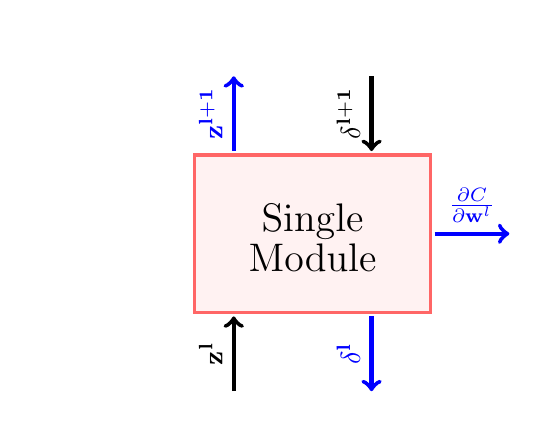
\begin{tikzpicture}[thick,scale=1, every node/.style={scale=1}]
    \node (B) at (3,0) {};

    \node (x1) at (1,3.5) {};
    \node (x2) at (1,2) {};
    \node (x3) at (1,0.5) {};
    \node (x4) at (1,-1) {};


    \filldraw[color=red!60, fill=red!5, very thick,](B) rectangle +(3,2) node {};
    \draw (B)+(1.5,1.15) node {\Large{Single}};
    \draw (B)+(1.5,0.7) node {\Large{Module}};

  
    \draw[ultra thick, ->] (3.5,-1) -> (3.5,-0.05) node [pos=0.5,above,rotate=90] (TextNode) {$\mathbf{z^{l}}$};    
    \draw[ultra thick,blue, ->] (5.25,-0.05) -> (5.25,-1) node [pos=0.5,above,rotate=90] (TextNode) {$\mathbf{\delta^{l}}$};  

    \draw[ultra thick,blue, ->] (3.5,2.05) -> (3.5,3) node [pos=0.5,above,rotate=90] (TextNode) {$\mathbf{z^{l+1}}$};
    \draw[ultra thick, ->] (5.25,3) -> (5.25,2.05) node [pos=0.5,above,rotate=90] (TextNode) {$\mathbf{\delta^{l+1}}$};

    \draw[ultra thick,blue, ->] (6.05,1) -> (7,1) node [pos=0.5,above] (TextNode) {$\frac{\partial C}{\partial\mathbf{w}^{l}}$};



  \end{tikzpicture}
\end{centering}

\end{document}